\chapter{Language server}

The purpose of Language server is to implement the Language Server Protocol and Debug Adapter Protocol and to provide access to parser library using these protocols. It has to deserialize and serialize LSP and DAP messages, keep them in the right order and then serve all the requests by invoking parser library.

\section{LSP}
short overview of LSP

definition of message, notification, request
\section{DAP}
short overview of DAP

\section{Third party libraries}
Language server uses three third party libraries: ASIO C++ library \footnote{\url{https://think-async.com/Asio/}}, JSON for Modern C++ \footnote{\url{https://github.com/nlohmann/json}} and 
cpp-netlib URI \footnote{\url{https://github.com/cpp-netlib/uri}}.

\subsection{ASIO C++ library}
Asio is a cross-platform C++ library for network and low-level I/O programming that provides developers with a consistent asynchronous model using a modern C++ approach. We use it to handle TCP communication in a cross-platform way. Asio implements std::iostream wrappers around the TCP stream, which allows us to abstract from the actual source of the communication.

\subsection{JSON for Modern C++}
We use the JSON for Modern C++ library to parse and serialize json, it is used in both LSP and DAP. It allows us to seamlessly traverse input json and extract the interesting values as well as easily respond with valid json messages.

\subsection{cpp-netlib URI}
Cpp-netlib URI library supports URI specified by the RFC3986 \footnote{\url{https://tools.ietf.org/html/rfc3986}}, which is used by the LSP and DAP protocols to transfer paths to files. It is the responsibility of language server to parse the URIs and convert them to file paths, so it is easier to work with them in the parser library. 

\section{Language server overview}
The architecture of the Language server component is illustrated in \cref{lang_server_arch}. It communicates on standard input/output by LSP with LSP client and listens on a TCP port to provide DAP support for macro tracer. The TCP communication is wrapped by class \TT{TCP handler}, which uses boost::asio library to provide the TCP communication as common C++ iostream.


\begin{figure}
	\centering
	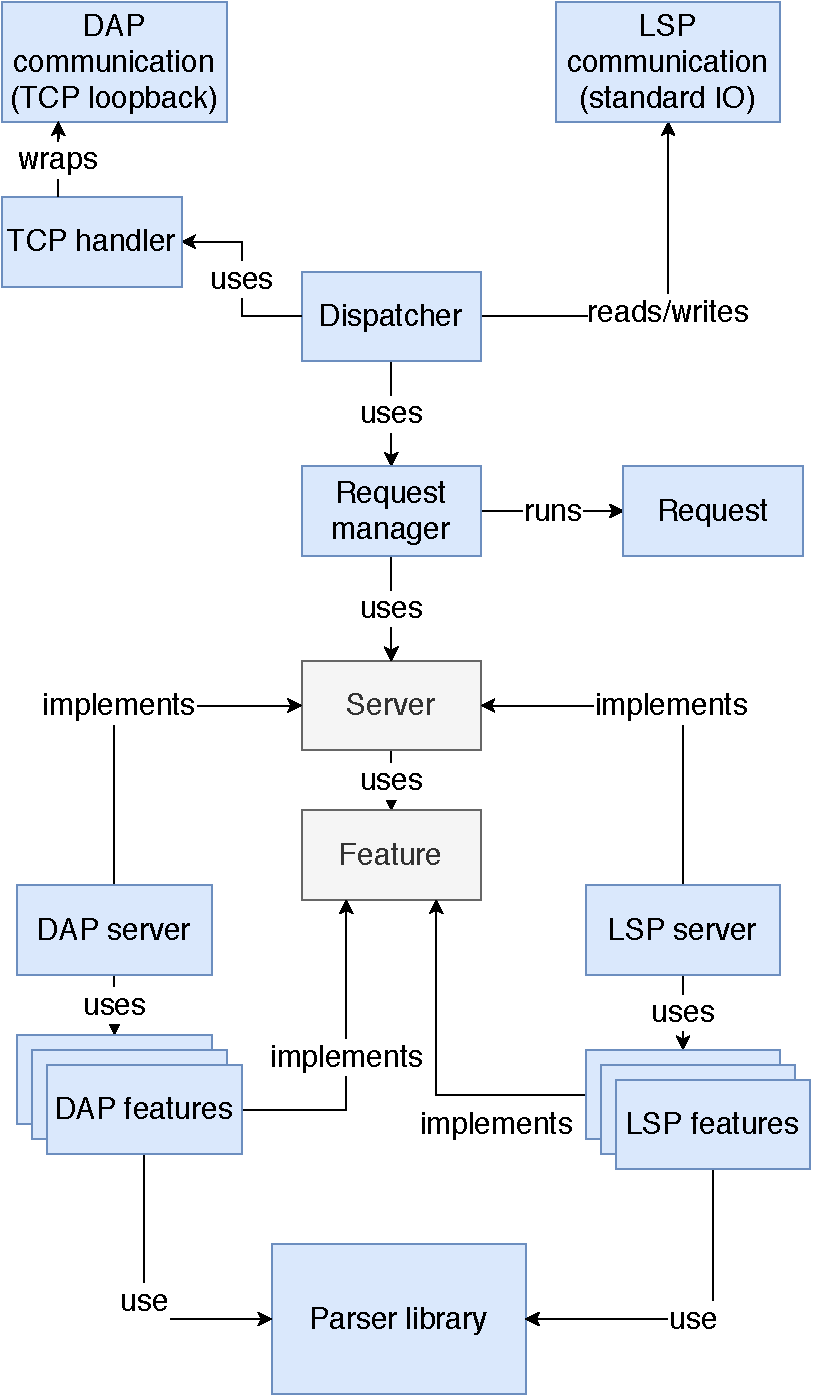
\includegraphics[width=11cm]{img/lang_server}
	\caption{Architecture of language server.}
	\label{lang_server_arch}
\end{figure}


The main purpose of the \TT{Dispatcher} is to provide abstraction for the lowest level communication, which is shared by LSP and DAP. It reads iostream to parse messages using the JSON for Modern C++ library and stores them in \TT{request manager} as requests.

A \TT{request} encapsulates one message that came from the client and basically is represented only by raw (but parsed) json.

\TT{Request manager} stores \TT{requests} in a queue and runs a worker thread that serves the requests one by one. There is only one instance of request manager running in the language server, so it serializes requests from DAP and LSP (which come asynchronously from separate sources) into one queue.

\TT{Server} is an abstract class that implements protocol behaviour that is common for both DAP and LSP --- it basically implements Remote Procedure Call. Actual handling of LSP and DAP requests is implemented in \TT{features}. Each \TT{feature} contains implementation of several protocol requests or notifications. The \TT{features} unwrap the arguments from json and call corresponding parser library methods.

Both LSP and DAP have their implementation of the abstract \TT{server} class. They both implement the initialization and finalization of protocol communication, which is a bit different for both protocols and both use \TT{features} to serve protocol requests.


\section{I/O handling}
The dispatcher purpose is to abstract from the complexity of working with raw strings and streams. It runs an infinite loop in which it reads messages from std::iostream and adds them to request manager as parsed json objects. At the same time, it is able to write responses in the correct format.

The language server communicates with LSP client on standard input and output, so we simply use the \TT{dispatcher} with the standard std::iostream class to communicate with the LSP client.

The DAP communicates with TCP, which is less straightforward. The extension finds a free TCP port just before it starts the language server and passes it as argument to the executable. The \TT{TCP handler} then starts listening on that port. Once the user wants to start macro tracer, the DAP client connects to the port on localhost and the \TT{TCP handler} accepts the TCP client and starts \TT{dispatcher} and \TT{DAP server}. Once the DAP communication ends, both \TT{dispatcher} and \TT{DAP server} are destroyed and \TT{TCP handler} listens again for next DAP session. Thanks to the ASIO library implementation of the std::iostream interface, the dispatcher is able to completely abstract from the fact that it is communicating through TCP and not standard IO.

\section{Servers}
The servers are able to process incoming LSP and DAP requests. They get the messages in the form of already parsed jsons. Then they extract the name of requested method from the message and call corresponding method.

There are two server classes: \TT{LSP server} and \TT{DAP server}, which both inherit from abstract class \TT{server}. They implement protocol-specific processing of messages --- although the protocols are quite similar, each protocol has different initialization and finalization, different message format, etc.

The functionality of servers is divided in features. Each feature implements several LSP or DAP methods by unpacking the arguments of the method and calling corresponding parser library function. At initialization, each feature adds its methods to the server's list of implemented methods. The LSP server uses three features:
\begin{itemize}
	\item Text synchronization feature, which handles the notifications about state of opened files in the editor
	\item Workspace folders feature, which handles the notifications about adding and removing workspaces.
	\item Language feature, which handles requests of HLASM code information.
\end{itemize}
The \cref{LSP_methods} shows the list of all implemented LSP methods and the class where the implementation lies.

\begin{longtable}{ll}
	\caption{The list of all implemented LSP methods and the classes where they are implemented}
	\label{LSP_methods}   \\ \toprule
	\textbf{LSP Method name} & \textbf{Component} \\ \midrule
	initialize  & LSP server     \\
	shutdown    & LSP server     \\
	exit        & LSP server    \\
	textDocument/publishDiagnostics & LSP server \\
	textDocument/didOpen  &  Text synchronization feature    \\
	textDocument/didChange  & Text synchronization feature     \\
	textDocument/didClose  &  Text synchronization feature    \\
	textDocument/semanticHighlighting & Text synchronization feature \\
	workspace/didChangeWorkspaceFolders  & Workspace folders feature     \\
	workspace/didChangeWatchedFiles  & Workspace folders feature     \\
	textDocument/definition  & Language feature     \\
	textDocument/references  & Language feature     \\
	textDocument/hover  & Language feature     \\
	textDocument/completion  & Language feature     \\ \bottomrule
\end{longtable}

The DAP server uses only one feature: Launch feature, which handles stepping through the code and retrieving information about variables and stack trace. The table \cref{DAP_methods} shows the list of all implemented DAP methods.

\begin{longtable}{ll}
	\caption{The list of all implemented DAP methods and the classes where they are implemented}
	\label{DAP_methods}   \\ \toprule
	\textbf{LSP Method name} & \textbf{Component} \\ \midrule
	initialize  & LSP server     \\
	disconnect    & LSP server     \\
	launch & Launch feature \\
	setBreakpoints  &  Launch feature    \\
	configurationDone  & Launch feature     \\
	threads  &  Launch feature    \\
	stackTrace & Launch feature \\
	scopes  & Launch feature     \\
	next  & Launch feature     \\
	stepIn  & Launch feature     \\
	variables  & Launch feature     \\
	continue  & Launch feature \\
 stopped & Launch feature \\
 exited  & Launch feature \\
 terminated & Launch feature \\\bottomrule
\end{longtable}

\section{result respond}

\section{Request Manager}

Request manager encapsulates a queue of requests with a worker thread that processes those requests. There may be up to two dispatcher instances in the language server: one for LSP and one for DAP. Both of them add the requests they parse into one request manager. It is necessary to process the requests one by one, because the parser library cannot process more requests at the same time.

There are three threads running in the language server:
\begin{enumerate}
	\item LSP read thread --- a thread in which Dispatcher reads messages from standard input
	\item DAP read thread --- a thread in which TCP handler listens on a localhost port to initiate DAP session. After accepting the DAP client, the dispatcher reads DAP input on this thread too.
	\item Worker thread in\TT{request manager} that processes each request using \TT{LSP server} or \TT{DAP server} and ultimately the parser library.
\end{enumerate}

The threads are synchronized in two ways: first, there is a mutex that protects adding to the request queue simultaneously by the LSP and DAP read threads. Second, there is a conditional variable to control the worker thread so it sleeps when there are no requests and wakes up when a new request has been added.

In request manager, there is a mechanism for invalidating requests that have been obsoleted by a new requests.


\section{Example: hover request handling}

\begin{landscape}
	\begin{figure}
		\centering
		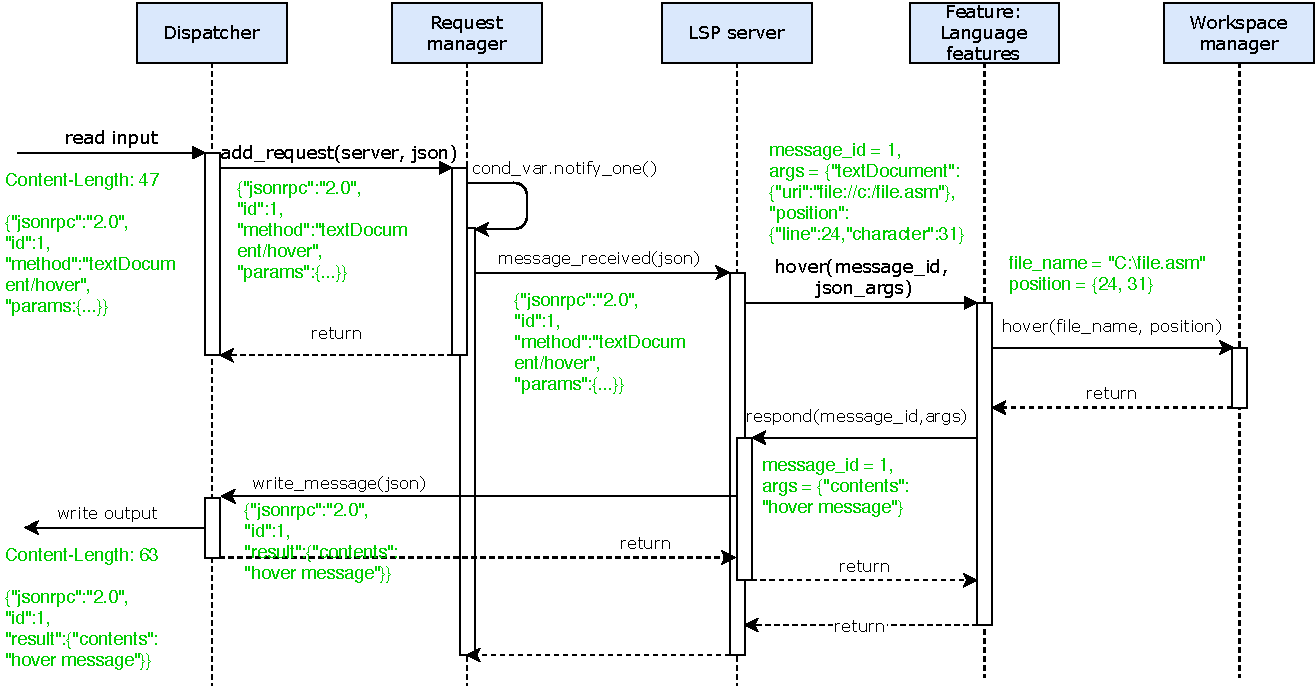
\includegraphics[width=21cm]{img/hover_sequence}
		\caption{Sequence diagram showing processing of the textDocument/hover request in the language server}
		\label{lang_server_arch}
	\end{figure}
\end{landscape}
